% Cuanto mejora el trapecio. GENERADO por figuras_mejora.py: no editar a mano.
\documentclass[border=0pt,tikz]{standalone}
\usepackage[utf8]{inputenc}
\usepackage[T1]{fontenc}
\usepackage{lmodern}
\usepackage{amsmath}
\usepackage[none]{hyphenat}
% Estilo común de las figuras TikZ (panoramas y diagramas de bloques).
%
% Cada figura lo incluye con \input{../../figuras/estilo_tikz.tex} (las figuras
% viven en docs/<módulo>/figuras/). Un solo lugar para la paleta, los estilos de
% bloque y el formato de los parámetros: si cambia algo acá, cambia en todas.
%
% La paleta es la misma de docs/figuras/estilo_svg.py y de PALETA en
% modulos/mk/datasheet.py; si se toca un color, se toca en los tres.
%
% Requiere: \usepackage{tikz} (lo da la clase standalone con la opción tikz).

\usetikzlibrary{arrows.meta,positioning,calc,fit,backgrounds,shapes.multipart,
                decorations.markings,shadows}

% ---------------------------------------------------------------- colores ---
\definecolor{azul}{RGB}{108,172,228}      % acondicionamiento
\definecolor{verde}{RGB}{110,214,142}     % captura / histogramas en BRAM
\definecolor{amarillo}{RGB}{252,232,160}  % trigger
\definecolor{naranja}{RGB}{252,206,160}   % camino a DDR
\definecolor{grisr}{RGB}{226,226,226}     % compartido / infraestructura
\definecolor{rojo}{RGB}{240,128,128}      % bus del sistema

% ---------------------------------------------------------------- estilos ---
\tikzset{
  >={Stealth[length=2.4mm,width=1.8mm]},
  % fondo blanco siempre: el SVG se ve igual en modo claro y oscuro
  fondo/.style   = {show background rectangle, inner frame sep=8pt,
                    background rectangle/.style={fill=white, draw=none}},
  bloque/.style  = {draw=black, line width=0.6pt, rounded corners=2pt,
                    align=center, text width=2.2cm, minimum height=1.15cm,
                    inner sep=2pt, font=\scriptsize, fill=#1},
  datos/.style   = {bloque=azul!35},
  trig/.style    = {bloque=amarillo},
  captura/.style = {bloque=verde!55},
  ddr/.style     = {bloque=naranja!70},
  comp/.style    = {bloque=grisr},
  bus/.style     = {bloque=rojo!45},
  % lógica escrita dentro del módulo, sin submódulo propio
  etapa/.style   = {bloque=#1, line width=0.5pt},
  etapa/.default = verde!20,
  % lo que el bitstream no trae (atado a cero, stub, salida muda)
  mudo/.style    = {bloque=white, draw=black!45, dashed, text=black!55},
  %
  % BLOQUE CON PARÁMETROS, en el formato del datasheet: el encabezado lleva el
  % nombre y los parámetros con que lo instancia el padre (NOMBRE=valor, en
  % monoespaciada, uno por línea); el cuerpo, más claro, lo que hace.
  %   \node[datos, param={azul!35}{azul!12}] {\blk{nombre}{} \prm{A=1\\B=2}
  %                                            \nodepart{two} función};
  param/.style 2 args = {rectangle split, rectangle split parts=2,
                         rectangle split part fill={#1, #2}},
  %
  flujo/.style   = {->, line width=0.8pt},
  ctrl/.style    = {->, line width=0.6pt, black!65},
  % la línea que pasa por encima en un cruce: un halo blanco la separa
  cruce/.style   = {preaction={draw=white, line width=3.4pt, -}},
  % marca de ancho de bus: barra oblicua a mitad de la flecha, con el número
  % encima. \draw[flujo, ancho=14] ...; para otra posición, ancho en=0.3.
  ancho/.style   = {decoration={markings, mark=at position \anchopos with {
                      \draw[line width=0.6pt, -] (-0.1,-0.14) -- (0.1,0.14);
                      \node[font=\scriptsize, above=1.5pt] {#1};}},
                    postaction={decorate}},
  % la misma marca en una flecha vertical: el número va a la derecha
  anchov/.style  = {decoration={markings, mark=at position \anchopos with {
                      \draw[line width=0.6pt, -] (-0.14,-0.1) -- (0.14,0.1);
                      \node[font=\scriptsize, right=3pt] {#1};}},
                    postaction={decorate}},
  ancho en/.code = {\def\anchopos{#1}},
  sen/.style     = {font=\scriptsize\ttfamily, inner sep=1.5pt},
  nodo/.style    = {font=\tiny\ttfamily, inner sep=1pt, black!75},
  pin/.style     = {font=\scriptsize, align=center, inner sep=1pt},
  grupo/.style   = {draw=black!55, dashed, line width=0.7pt, rounded corners=4pt},
  canal/.style   = {grupo},
  contenedor/.style = {draw=black!80, line width=1.0pt, rounded corners=6pt},
  % marca numerada: cada número es una fila de la tabla del documento
  marca/.style   = {circle, fill=black, text=white, font=\scriptsize\bfseries,
                    inner sep=0pt, minimum size=4.3mm},
  %
  % DECISIONES (docs/mca/vista_general_mca.md). Cada opción es un bloque, todas
  % entran a un mux (\muxdec, abajo) y el registro que elige entra por abajo.
  % la opción que trae el reset (el comportamiento histórico): borde doble
  defecto/.style = {double=white, double distance=0.8pt, line width=0.45pt},
  % rótulo de la decisión, el mismo Dn del panorama y del documento
  decision/.style = {circle, fill=black, text=white, font=\small\bfseries,
                     inner sep=0pt, minimum size=7mm},
  %
  % LÓGICA (docs/mca/figuras/contabilidad/ y los detalles de las decisiones)
  % registro: caja gris con el triángulo de reloj en el borde de abajo
  registro/.style = {draw=black, line width=0.6pt, fill=grisr, align=center,
                     font=\scriptsize, inner sep=2pt, minimum width=#1,
                     minimum height=0.85cm,
                     path picture={\draw[line width=0.5pt]
                       ([xshift=-1.1mm]path picture bounding box.south) --
                       ([yshift=1.6mm]path picture bounding box.south) --
                       ([xshift=1.1mm]path picture bounding box.south);}},
  registro/.default = 0.8cm,
  % condición de una cadena if / else-if: "sí" sale a la derecha, "no" abajo
  pregunta/.style = {draw=black, line width=0.5pt, rounded corners=7pt,
                     fill=white, font=\scriptsize\ttfamily, align=center,
                     inner sep=2.5pt, minimum height=0.62cm, text width=#1},
  pregunta/.default = 1.9cm,
  si/.style      = {font=\tiny, inner sep=1pt, above, pos=0.12},
  no/.style      = {font=\tiny, inner sep=1pt, left, pos=0.45},
  %
  titulo/.style  = {anchor=north west, font=\small, inner sep=4pt, align=left},
  rotulo/.style  = {anchor=north west, font=\scriptsize\itshape, black!70,
                    inner sep=2pt, align=left},
}

% submódulo: nombre en monoespaciada; lógica propia: nombre en romana
\newcommand{\blk}[2]{{\ttfamily\bfseries #1}\\[1pt]#2}
\newcommand{\etq}[2]{{\bfseries #1}\\[1pt]#2}
\newcommand{\punto}[1]{\fill (#1) circle (1.3pt);}

% Parámetros en el formato del datasheet: NOMBRE=valor en monoespaciada, una
% entrada por celda, hasta cuatro columnas. Una columna: \prm{A=1\\B=2};
% dos: \prm{A=1 & B=2\\C=3}.
\newcommand{\prm}[1]{{\ttfamily\fontsize{5.6}{6.6}\selectfont
  \begin{tabular}{@{}l@{\hspace{7pt}}l@{\hspace{7pt}}l@{\hspace{7pt}}l@{}}#1\end{tabular}}}

\def\anchopos{0.5}

% Mux de una decisión: trapecio con el lado ancho (las entradas) a la izquierda.
% #1 = nombre, #2 = centro, #3 = alto en cm. Deja tres coordenadas:
%   (#1-in)  centro del lado de entradas: las flechas llegan a (#1-in |- opcion.east)
%   (#1-out) la salida
%   (#1-sel) mitad del lado de abajo: por ahí entra el registro que elige
% El rótulo de adentro es opcional: \muxdec{m}{(4,0)}{3.6} y después
% \node[...] at (m) {...}.
\newcommand{\muxdec}[3]{%
  \path #2 coordinate (#1);
  \draw[line width=0.6pt, fill=grisr]
    ($(#1)+(-0.45,{#3/2})$) -- ($(#1)+(0.45,{#3/2-0.35})$) --
    ($(#1)+(0.45,{-#3/2+0.35})$) -- ($(#1)+(-0.45,{-#3/2})$) -- cycle;
  \coordinate (#1-in)  at ($(#1)+(-0.45,0)$);
  \coordinate (#1-out) at ($(#1)+(0.45,0)$);
  \coordinate (#1-sel) at ($(#1)+(0,{-#3/2+0.175})$);}

% El mismo mux rotado 90 grados, para un flujo de arriba hacia abajo: entradas
% por el lado ancho de arriba, salida abajo y el registro que elige por la
% izquierda. #1 = nombre, #2 = centro, #3 = ancho en cm. Deja (#1-in) centro del
% lado de entradas, (#1-out) la salida y (#1-sel) mitad del lado izquierdo.
\newcommand{\muxdecv}[3]{%
  \path #2 coordinate (#1);
  \draw[line width=0.6pt, fill=grisr]
    ($(#1)+({-#3/2},0.45)$) -- ($(#1)+({#3/2},0.45)$) --
    ($(#1)+({#3/2-0.35},-0.45)$) -- ($(#1)+({-#3/2+0.35},-0.45)$) -- cycle;
  \coordinate (#1-in)  at ($(#1)+(0,0.45)$);
  \coordinate (#1-out) at ($(#1)+(0,-0.45)$);
  \coordinate (#1-sel) at ($(#1)+({-#3/2+0.175},0)$);}

% Leyenda de colores + nota. #1 = posición, #2 = color/texto, #3 = nota.
\newcommand{\leyenda}[3]{%
  \begin{scope}[shift={(#1)}, every node/.style={font=\scriptsize}]
    \coordinate (t0) at (-0.5,0);
    \foreach \c/\t [count=\i] in {#2} {
      \pgfmathtruncatemacro\j{\i-1}
      \node[draw, fill=\c, minimum width=4mm, minimum height=3mm, inner sep=0pt,
            right=5mm of t\j.east, anchor=west] (l\i) {};
      \node[right=1.5mm of l\i] (t\i) {\t};
    }
    \node[anchor=north west, black!70, text width=19cm, align=left]
      at (-0.05,-0.3) {#3};
  \end{scope}}

% Lo que dicen los parámetros, para la nota de la leyenda
\newcommand{\notaparam}{\texttt{NOMBRE=valor}: parámetros con que el padre
  instancia el bloque (se omiten los que sólo pasan el del padre sin cambio).}

\begin{document}
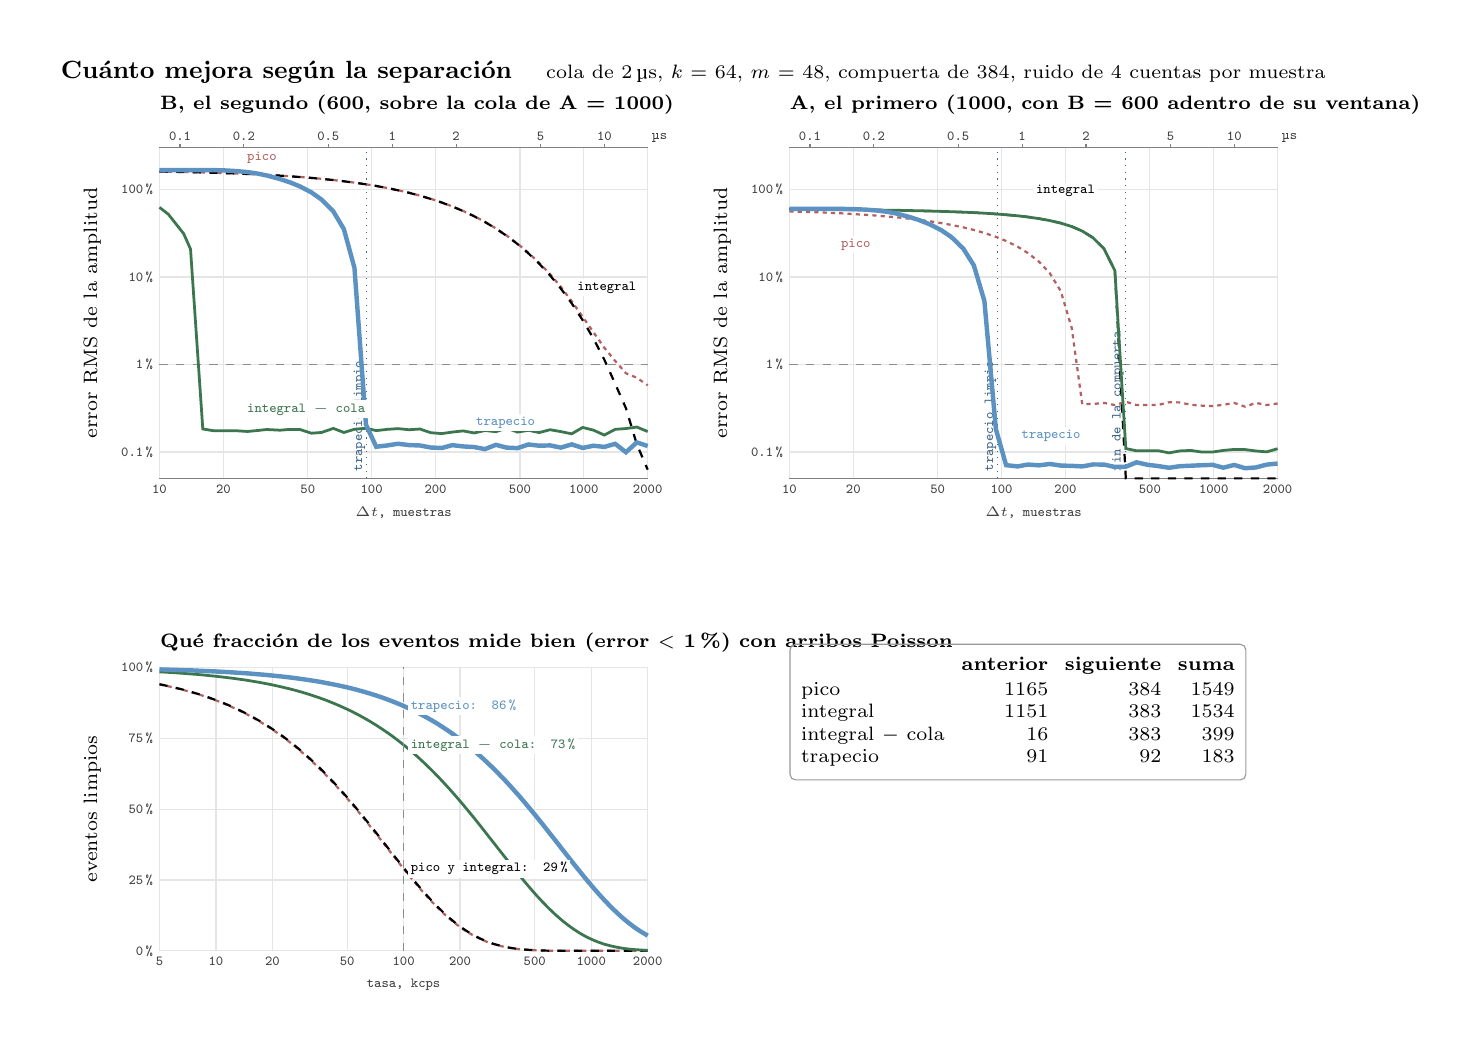
\begin{tikzpicture}[fondo]
\node[titulo] at (-1.4,6.45) {\textbf{Cuánto mejora según la separación} \quad {\scriptsize cola de 2\,µs, $k$ = 64, $m$ = 48, compuerta de 384, ruido de 4 cuentas por muestra}};
\node[anchor=south west, font=\scriptsize\bfseries, inner sep=0pt] at (0.000,5.620) {B, el segundo (600, sobre la cola de A = 1000)};
\draw[black!50, line width=0.4pt] (0.000,1.000) rectangle (6.200,5.200);
\draw[black!10] (0.000,1.335) -- (6.200,1.335);
\node[nodo, anchor=east] at (-0.040,1.335) {0.1\,\%};
\draw[black!10] (0.000,2.446) -- (6.200,2.446);
\node[nodo, anchor=east] at (-0.040,2.446) {1\,\%};
\draw[black!10] (0.000,3.558) -- (6.200,3.558);
\node[nodo, anchor=east] at (-0.040,3.558) {10\,\%};
\draw[black!10] (0.000,4.670) -- (6.200,4.670);
\node[nodo, anchor=east] at (-0.040,4.670) {100\,\%};
\draw[black!10] (0.000,1.000) -- (0.000,5.200);
\node[nodo, anchor=north] at (0.000,0.960) {10};
\draw[black!10] (0.811,1.000) -- (0.811,5.200);
\node[nodo, anchor=north] at (0.811,0.960) {20};
\draw[black!10] (1.883,1.000) -- (1.883,5.200);
\node[nodo, anchor=north] at (1.883,0.960) {50};
\draw[black!10] (2.694,1.000) -- (2.694,5.200);
\node[nodo, anchor=north] at (2.694,0.960) {100};
\draw[black!10] (3.506,1.000) -- (3.506,5.200);
\node[nodo, anchor=north] at (3.506,0.960) {200};
\draw[black!10] (4.578,1.000) -- (4.578,5.200);
\node[nodo, anchor=north] at (4.578,0.960) {500};
\draw[black!10] (5.389,1.000) -- (5.389,5.200);
\node[nodo, anchor=north] at (5.389,0.960) {1000};
\draw[black!10] (6.200,1.000) -- (6.200,5.200);
\node[nodo, anchor=north] at (6.200,0.960) {2000};
\node[nodo, anchor=north] at (3.100,0.680) {$\Delta t$, muestras};
\node[font=\scriptsize, anchor=south, rotate=90] at (-0.620,3.100) {error RMS de la amplitud};
\draw[black!50] (0.261,5.200) -- ++(0,0.05) node[above, nodo] {0.1};
\draw[black!50] (1.072,5.200) -- ++(0,0.05) node[above, nodo] {0.2};
\draw[black!50] (2.144,5.200) -- ++(0,0.05) node[above, nodo] {0.5};
\draw[black!50] (2.956,5.200) -- ++(0,0.05) node[above, nodo] {1};
\draw[black!50] (3.767,5.200) -- ++(0,0.05) node[above, nodo] {2};
\draw[black!50] (4.839,5.200) -- ++(0,0.05) node[above, nodo] {5};
\draw[black!50] (5.650,5.200) -- ++(0,0.05) node[above, nodo] {10};
\node[nodo, anchor=west] at (6.220,5.320) {µs};
\draw[black!45, dashed] (0.000,2.446) -- (6.200,2.446);
\draw[azul!60!black, line width=0.4pt, dotted] (2.634,1.000) -- (2.634,5.200);
\node[nodo, anchor=south west, text=azul!60!black, rotate=90] at (2.654,1.050) {trapecio limpio};
\draw[rojo!75!black, line width=0.8pt, dash pattern=on 1.5pt off 1.5pt] plot coordinates {(0.000,4.897) (0.112,4.895) (0.307,4.891) (0.394,4.890) (0.550,4.886) (0.688,4.882) (0.811,4.878) (0.975,4.872) (1.118,4.866) (1.246,4.860) (1.361,4.855) (1.531,4.845) (1.651,4.837) (1.786,4.828) (1.929,4.816) (2.057,4.805) (2.208,4.789) (2.342,4.774) (2.476,4.756) (2.622,4.735) (2.752,4.714) (2.898,4.687) (3.028,4.660) (3.169,4.628) (3.308,4.591) (3.446,4.551) (3.585,4.504) (3.719,4.454) (3.857,4.396) (3.996,4.331) (4.133,4.259) (4.272,4.175) (4.409,4.084) (4.547,3.981) (4.685,3.866) (4.822,3.736) (4.960,3.595) (5.098,3.431) (5.235,3.250) (5.374,3.052) (5.511,2.857) (5.649,2.660) (5.787,2.492) (5.924,2.335) (6.062,2.278) (6.200,2.182)};
\draw[black, line width=0.8pt, dashed] plot coordinates {(0.000,4.897) (0.112,4.895) (0.307,4.891) (0.394,4.889) (0.550,4.885) (0.688,4.882) (0.811,4.878) (0.975,4.872) (1.118,4.866) (1.246,4.860) (1.361,4.854) (1.531,4.845) (1.651,4.837) (1.786,4.827) (1.929,4.816) (2.057,4.804) (2.208,4.789) (2.342,4.773) (2.476,4.756) (2.622,4.735) (2.752,4.714) (2.898,4.686) (3.028,4.659) (3.169,4.627) (3.308,4.590) (3.446,4.549) (3.585,4.503) (3.719,4.453) (3.857,4.395) (3.996,4.329) (4.133,4.256) (4.272,4.173) (4.409,4.080) (4.547,3.976) (4.685,3.858) (4.822,3.727) (4.960,3.578) (5.098,3.410) (5.235,3.223) (5.374,3.010) (5.511,2.776) (5.649,2.509) (5.787,2.202) (5.924,1.891) (6.062,1.433) (6.200,1.111)};
\draw[verde!55!black, line width=1.0pt] plot coordinates {(0.000,4.442) (0.112,4.355) (0.307,4.108) (0.394,3.912) (0.550,1.628) (0.688,1.605) (0.811,1.606) (0.975,1.605) (1.118,1.596) (1.246,1.608) (1.361,1.621) (1.531,1.612) (1.651,1.622) (1.786,1.620) (1.929,1.574) (2.057,1.583) (2.208,1.635) (2.342,1.583) (2.476,1.624) (2.622,1.636) (2.752,1.607) (2.898,1.623) (3.028,1.632) (3.169,1.618) (3.308,1.627) (3.446,1.580) (3.585,1.569) (3.719,1.588) (3.857,1.603) (3.996,1.577) (4.133,1.608) (4.272,1.593) (4.409,1.638) (4.547,1.588) (4.685,1.611) (4.822,1.582) (4.960,1.618) (5.098,1.594) (5.235,1.566) (5.374,1.647) (5.511,1.613) (5.649,1.550) (5.787,1.623) (5.924,1.633) (6.062,1.652) (6.200,1.595)};
\draw[azul!85!black, line width=1.6pt] plot coordinates {(0.000,4.916) (0.112,4.916) (0.307,4.916) (0.394,4.916) (0.550,4.916) (0.688,4.915) (0.811,4.912) (0.975,4.903) (1.118,4.890) (1.246,4.871) (1.361,4.847) (1.531,4.802) (1.651,4.762) (1.786,4.707) (1.929,4.632) (2.057,4.542) (2.208,4.390) (2.342,4.165) (2.476,3.673) (2.622,1.683) (2.752,1.402) (2.898,1.419) (3.028,1.440) (3.169,1.423) (3.308,1.418) (3.446,1.392) (3.585,1.386) (3.719,1.422) (3.857,1.406) (3.996,1.398) (4.133,1.372) (4.272,1.426) (4.409,1.391) (4.547,1.384) (4.685,1.431) (4.822,1.415) (4.960,1.419) (5.098,1.391) (5.235,1.432) (5.374,1.387) (5.511,1.415) (5.649,1.400) (5.787,1.439) (5.924,1.332) (6.062,1.457) (6.200,1.411)};
\node[nodo, anchor=south west, text=rojo!75!black, fill=white, inner sep=1pt] at (1.072,4.953) {pico};
\node[nodo, anchor=south west, text=verde!55!black, fill=white, inner sep=1pt] at (1.072,1.757) {integral $-$ cola};
\node[nodo, anchor=south west, text=azul!85!black, fill=white, inner sep=1pt] at (3.980,1.591) {trapecio};
\node[nodo, anchor=south west, text=black, fill=white, inner sep=1pt] at (5.266,3.311) {integral};
\node[anchor=south west, font=\scriptsize\bfseries, inner sep=0pt] at (8.000,5.620) {A, el primero (1000, con B = 600 adentro de su ventana)};
\draw[black!50, line width=0.4pt] (8.000,1.000) rectangle (14.200,5.200);
\draw[black!10] (8.000,1.335) -- (14.200,1.335);
\node[nodo, anchor=east] at (7.960,1.335) {0.1\,\%};
\draw[black!10] (8.000,2.446) -- (14.200,2.446);
\node[nodo, anchor=east] at (7.960,2.446) {1\,\%};
\draw[black!10] (8.000,3.558) -- (14.200,3.558);
\node[nodo, anchor=east] at (7.960,3.558) {10\,\%};
\draw[black!10] (8.000,4.670) -- (14.200,4.670);
\node[nodo, anchor=east] at (7.960,4.670) {100\,\%};
\draw[black!10] (8.000,1.000) -- (8.000,5.200);
\node[nodo, anchor=north] at (8.000,0.960) {10};
\draw[black!10] (8.811,1.000) -- (8.811,5.200);
\node[nodo, anchor=north] at (8.811,0.960) {20};
\draw[black!10] (9.883,1.000) -- (9.883,5.200);
\node[nodo, anchor=north] at (9.883,0.960) {50};
\draw[black!10] (10.694,1.000) -- (10.694,5.200);
\node[nodo, anchor=north] at (10.694,0.960) {100};
\draw[black!10] (11.506,1.000) -- (11.506,5.200);
\node[nodo, anchor=north] at (11.506,0.960) {200};
\draw[black!10] (12.578,1.000) -- (12.578,5.200);
\node[nodo, anchor=north] at (12.578,0.960) {500};
\draw[black!10] (13.389,1.000) -- (13.389,5.200);
\node[nodo, anchor=north] at (13.389,0.960) {1000};
\draw[black!10] (14.200,1.000) -- (14.200,5.200);
\node[nodo, anchor=north] at (14.200,0.960) {2000};
\node[nodo, anchor=north] at (11.100,0.680) {$\Delta t$, muestras};
\node[font=\scriptsize, anchor=south, rotate=90] at (7.380,3.100) {error RMS de la amplitud};
\draw[black!50] (8.261,5.200) -- ++(0,0.05) node[above, nodo] {0.1};
\draw[black!50] (9.072,5.200) -- ++(0,0.05) node[above, nodo] {0.2};
\draw[black!50] (10.144,5.200) -- ++(0,0.05) node[above, nodo] {0.5};
\draw[black!50] (10.956,5.200) -- ++(0,0.05) node[above, nodo] {1};
\draw[black!50] (11.767,5.200) -- ++(0,0.05) node[above, nodo] {2};
\draw[black!50] (12.839,5.200) -- ++(0,0.05) node[above, nodo] {5};
\draw[black!50] (13.650,5.200) -- ++(0,0.05) node[above, nodo] {10};
\node[nodo, anchor=west] at (14.220,5.320) {µs};
\draw[black!45, dashed] (8.000,2.446) -- (14.200,2.446);
\draw[azul!60!black, line width=0.4pt, dotted] (10.647,1.000) -- (10.647,5.200);
\node[nodo, anchor=south west, text=azul!60!black, rotate=90] at (10.667,1.050) {trapecio limpio};
\draw[azul!60!black, line width=0.4pt, dotted] (12.269,1.000) -- (12.269,5.200);
\node[nodo, anchor=south west, text=azul!60!black, rotate=90] at (12.289,1.050) {fin de la compuerta};
\draw[rojo!75!black, line width=0.8pt, dash pattern=on 1.5pt off 1.5pt] plot coordinates {(8.000,4.391) (8.112,4.387) (8.307,4.381) (8.394,4.378) (8.550,4.371) (8.688,4.365) (8.811,4.357) (8.975,4.347) (9.118,4.336) (9.246,4.326) (9.361,4.316) (9.531,4.297) (9.651,4.283) (9.786,4.265) (9.929,4.242) (10.057,4.219) (10.208,4.188) (10.342,4.155) (10.476,4.117) (10.622,4.068) (10.752,4.015) (10.898,3.943) (11.028,3.862) (11.169,3.753) (11.308,3.604) (11.446,3.378) (11.585,2.912) (11.719,1.943) (11.857,1.945) (11.996,1.959) (12.133,1.931) (12.272,1.974) (12.409,1.931) (12.547,1.932) (12.685,1.933) (12.822,1.967) (12.960,1.965) (13.098,1.934) (13.235,1.924) (13.374,1.918) (13.511,1.935) (13.649,1.958) (13.787,1.911) (13.924,1.959) (14.062,1.932) (14.200,1.951)};
\draw[black, line width=0.8pt, dashed] plot coordinates {(8.000,4.417) (8.112,4.417) (8.307,4.416) (8.394,4.415) (8.550,4.414) (8.688,4.413) (8.811,4.412) (8.975,4.410) (9.118,4.408) (9.246,4.406) (9.361,4.404) (9.531,4.401) (9.651,4.399) (9.786,4.395) (9.929,4.391) (10.057,4.387) (10.208,4.381) (10.342,4.375) (10.476,4.368) (10.622,4.358) (10.752,4.348) (10.898,4.335) (11.028,4.320) (11.169,4.300) (11.308,4.274) (11.446,4.242) (11.585,4.199) (11.719,4.141) (11.857,4.055) (11.996,3.915) (12.133,3.639) (12.272,1.000) (12.409,1.000) (12.547,1.000) (12.685,1.000) (12.822,1.000) (12.960,1.000) (13.098,1.000) (13.235,1.000) (13.374,1.000) (13.511,1.000) (13.649,1.000) (13.787,1.000) (13.924,1.000) (14.062,1.000) (14.200,1.000)};
\draw[verde!55!black, line width=1.0pt] plot coordinates {(8.000,4.417) (8.112,4.417) (8.307,4.416) (8.394,4.415) (8.550,4.414) (8.688,4.413) (8.811,4.412) (8.975,4.410) (9.118,4.408) (9.246,4.406) (9.361,4.405) (9.531,4.401) (9.651,4.399) (9.786,4.395) (9.929,4.391) (10.057,4.387) (10.208,4.381) (10.342,4.375) (10.476,4.368) (10.622,4.358) (10.752,4.348) (10.898,4.335) (11.028,4.320) (11.169,4.299) (11.308,4.274) (11.446,4.242) (11.585,4.199) (11.719,4.141) (11.857,4.055) (11.996,3.915) (12.133,3.639) (12.272,1.379) (12.409,1.350) (12.547,1.352) (12.685,1.351) (12.822,1.324) (12.960,1.349) (13.098,1.355) (13.235,1.335) (13.374,1.335) (13.511,1.355) (13.649,1.368) (13.787,1.366) (13.924,1.348) (14.062,1.337) (14.200,1.377)};
\draw[azul!85!black, line width=1.6pt] plot coordinates {(8.000,4.423) (8.112,4.423) (8.307,4.423) (8.394,4.423) (8.550,4.423) (8.688,4.422) (8.811,4.420) (8.975,4.413) (9.118,4.401) (9.246,4.385) (9.361,4.363) (9.531,4.318) (9.651,4.279) (9.786,4.225) (9.929,4.152) (10.057,4.065) (10.208,3.918) (10.342,3.706) (10.476,3.254) (10.622,1.626) (10.752,1.168) (10.898,1.152) (11.028,1.176) (11.169,1.166) (11.308,1.183) (11.446,1.163) (11.585,1.159) (11.719,1.152) (11.857,1.177) (11.996,1.175) (12.133,1.145) (12.272,1.148) (12.409,1.204) (12.547,1.173) (12.685,1.156) (12.822,1.135) (12.960,1.155) (13.098,1.161) (13.235,1.167) (13.374,1.172) (13.511,1.136) (13.649,1.171) (13.787,1.129) (13.924,1.139) (14.062,1.175) (14.200,1.189)};
\node[nodo, anchor=north east, text=rojo!75!black, fill=white, inner sep=1pt] at (9.072,4.088) {pico};
\node[nodo, anchor=south, text=black, fill=white, inner sep=1pt] at (11.506,4.531) {integral};
\node[nodo, anchor=south west, text=azul!85!black, fill=white, inner sep=1pt] at (10.908,1.423) {trapecio};
\node[anchor=south west, font=\scriptsize\bfseries, inner sep=0pt] at (0,-1.220) {Qué fracción de los eventos mide bien (error $<$ 1\,\%) con arribos Poisson};
\draw[black!50, line width=0.4pt] (0.000,-5.000) rectangle (6.200,-1.400);
\draw[black!10] (0.000,-5.000) -- (6.200,-5.000);
\node[nodo, anchor=east] at (-0.040,-5.000) {0\,\%};
\draw[black!10] (0.000,-4.100) -- (6.200,-4.100);
\node[nodo, anchor=east] at (-0.040,-4.100) {25\,\%};
\draw[black!10] (0.000,-3.200) -- (6.200,-3.200);
\node[nodo, anchor=east] at (-0.040,-3.200) {50\,\%};
\draw[black!10] (0.000,-2.300) -- (6.200,-2.300);
\node[nodo, anchor=east] at (-0.040,-2.300) {75\,\%};
\draw[black!10] (0.000,-1.400) -- (6.200,-1.400);
\node[nodo, anchor=east] at (-0.040,-1.400) {100\,\%};
\draw[black!10] (0.000,-5.000) -- (0.000,-1.400);
\node[nodo, anchor=north] at (0.000,-5.040) {5};
\draw[black!10] (0.717,-5.000) -- (0.717,-1.400);
\node[nodo, anchor=north] at (0.717,-5.040) {10};
\draw[black!10] (1.435,-5.000) -- (1.435,-1.400);
\node[nodo, anchor=north] at (1.435,-5.040) {20};
\draw[black!10] (2.383,-5.000) -- (2.383,-1.400);
\node[nodo, anchor=north] at (2.383,-5.040) {50};
\draw[black!10] (3.100,-5.000) -- (3.100,-1.400);
\node[nodo, anchor=north] at (3.100,-5.040) {100};
\draw[black!10] (3.817,-5.000) -- (3.817,-1.400);
\node[nodo, anchor=north] at (3.817,-5.040) {200};
\draw[black!10] (4.765,-5.000) -- (4.765,-1.400);
\node[nodo, anchor=north] at (4.765,-5.040) {500};
\draw[black!10] (5.483,-5.000) -- (5.483,-1.400);
\node[nodo, anchor=north] at (5.483,-5.040) {1000};
\draw[black!10] (6.200,-5.000) -- (6.200,-1.400);
\node[nodo, anchor=north] at (6.200,-5.040) {2000};
\node[nodo, anchor=north] at (3.100,-5.320) {tasa, kcps};
\node[font=\scriptsize, anchor=south, rotate=90] at (-0.620,-3.200) {eventos limpios};
\draw[rojo!75!black, line width=0.8pt, dash pattern=on 1.5pt off 1.5pt] plot coordinates {(0.000,-1.616) (0.078,-1.633) (0.157,-1.650) (0.235,-1.669) (0.314,-1.690) (0.392,-1.712) (0.471,-1.735) (0.549,-1.760) (0.628,-1.787) (0.706,-1.815) (0.785,-1.846) (0.863,-1.879) (0.942,-1.914) (1.020,-1.951) (1.099,-1.990) (1.177,-2.033) (1.256,-2.078) (1.334,-2.125) (1.413,-2.176) (1.491,-2.229) (1.570,-2.286) (1.648,-2.345) (1.727,-2.408) (1.805,-2.475) (1.884,-2.544) (1.962,-2.617) (2.041,-2.693) (2.119,-2.773) (2.197,-2.856) (2.276,-2.941) (2.354,-3.030) (2.433,-3.121) (2.511,-3.215) (2.590,-3.311) (2.668,-3.409) (2.747,-3.508) (2.825,-3.608) (2.904,-3.709) (2.982,-3.809) (3.061,-3.908) (3.139,-4.006) (3.218,-4.102) (3.296,-4.195) (3.375,-4.285) (3.453,-4.370) (3.532,-4.451) (3.610,-4.527) (3.689,-4.597) (3.767,-4.660) (3.846,-4.718) (3.924,-4.769) (4.003,-4.814) (4.081,-4.853) (4.159,-4.886) (4.238,-4.913) (4.316,-4.935) (4.395,-4.953) (4.473,-4.966) (4.552,-4.977) (4.630,-4.984) (4.709,-4.990) (4.787,-4.994) (4.866,-4.996) (4.944,-4.998) (5.023,-4.999) (5.101,-4.999) (5.180,-5.000) (5.258,-5.000) (5.337,-5.000) (5.415,-5.000) (5.494,-5.000) (5.572,-5.000) (5.651,-5.000) (5.729,-5.000) (5.808,-5.000) (5.886,-5.000) (5.965,-5.000) (6.043,-5.000) (6.122,-5.000) (6.200,-5.000)};
\draw[black, line width=0.8pt, dashed] plot coordinates {(0.000,-1.614) (0.078,-1.631) (0.157,-1.648) (0.235,-1.667) (0.314,-1.687) (0.392,-1.709) (0.471,-1.732) (0.549,-1.757) (0.628,-1.783) (0.706,-1.812) (0.785,-1.842) (0.863,-1.874) (0.942,-1.909) (1.020,-1.946) (1.099,-1.985) (1.177,-2.027) (1.256,-2.072) (1.334,-2.119) (1.413,-2.169) (1.491,-2.222) (1.570,-2.278) (1.648,-2.338) (1.727,-2.400) (1.805,-2.466) (1.884,-2.535) (1.962,-2.608) (2.041,-2.683) (2.119,-2.762) (2.197,-2.845) (2.276,-2.930) (2.354,-3.018) (2.433,-3.109) (2.511,-3.203) (2.590,-3.299) (2.668,-3.396) (2.747,-3.495) (2.825,-3.595) (2.904,-3.696) (2.982,-3.796) (3.061,-3.895) (3.139,-3.994) (3.218,-4.090) (3.296,-4.183) (3.375,-4.273) (3.453,-4.359) (3.532,-4.441) (3.610,-4.517) (3.689,-4.588) (3.767,-4.653) (3.846,-4.711) (3.924,-4.763) (4.003,-4.809) (4.081,-4.848) (4.159,-4.882) (4.238,-4.910) (4.316,-4.932) (4.395,-4.951) (4.473,-4.965) (4.552,-4.976) (4.630,-4.983) (4.709,-4.989) (4.787,-4.993) (4.866,-4.996) (4.944,-4.998) (5.023,-4.999) (5.101,-4.999) (5.180,-5.000) (5.258,-5.000) (5.337,-5.000) (5.415,-5.000) (5.494,-5.000) (5.572,-5.000) (5.651,-5.000) (5.729,-5.000) (5.808,-5.000) (5.886,-5.000) (5.965,-5.000) (6.043,-5.000) (6.122,-5.000) (6.200,-5.000)};
\draw[verde!55!black, line width=1.0pt] plot coordinates {(0.000,-1.457) (0.078,-1.461) (0.157,-1.466) (0.235,-1.471) (0.314,-1.477) (0.392,-1.483) (0.471,-1.489) (0.549,-1.496) (0.628,-1.504) (0.706,-1.512) (0.785,-1.521) (0.863,-1.530) (0.942,-1.540) (1.020,-1.551) (1.099,-1.562) (1.177,-1.575) (1.256,-1.588) (1.334,-1.603) (1.413,-1.618) (1.491,-1.635) (1.570,-1.653) (1.648,-1.672) (1.727,-1.692) (1.805,-1.714) (1.884,-1.738) (1.962,-1.763) (2.041,-1.790) (2.119,-1.819) (2.197,-1.850) (2.276,-1.883) (2.354,-1.918) (2.433,-1.955) (2.511,-1.995) (2.590,-2.038) (2.668,-2.083) (2.747,-2.131) (2.825,-2.182) (2.904,-2.235) (2.982,-2.292) (3.061,-2.353) (3.139,-2.416) (3.218,-2.482) (3.296,-2.552) (3.375,-2.626) (3.453,-2.702) (3.532,-2.782) (3.610,-2.865) (3.689,-2.951) (3.767,-3.040) (3.846,-3.132) (3.924,-3.226) (4.003,-3.322) (4.081,-3.420) (4.159,-3.520) (4.238,-3.620) (4.316,-3.720) (4.395,-3.820) (4.473,-3.920) (4.552,-4.017) (4.630,-4.113) (4.709,-4.206) (4.787,-4.295) (4.866,-4.380) (4.944,-4.460) (5.023,-4.535) (5.101,-4.604) (5.180,-4.667) (5.258,-4.724) (5.337,-4.775) (5.415,-4.819) (5.494,-4.857) (5.572,-4.889) (5.651,-4.916) (5.729,-4.937) (5.808,-4.954) (5.886,-4.968) (5.965,-4.978) (6.043,-4.985) (6.122,-4.990) (6.200,-4.994)};
\draw[azul!85!black, line width=1.6pt] plot coordinates {(0.000,-1.426) (0.078,-1.428) (0.157,-1.431) (0.235,-1.433) (0.314,-1.436) (0.392,-1.438) (0.471,-1.441) (0.549,-1.445) (0.628,-1.448) (0.706,-1.452) (0.785,-1.456) (0.863,-1.460) (0.942,-1.465) (1.020,-1.470) (1.099,-1.475) (1.177,-1.481) (1.256,-1.488) (1.334,-1.494) (1.413,-1.502) (1.491,-1.510) (1.570,-1.518) (1.648,-1.527) (1.727,-1.537) (1.805,-1.548) (1.884,-1.559) (1.962,-1.571) (2.041,-1.584) (2.119,-1.599) (2.197,-1.614) (2.276,-1.630) (2.354,-1.647) (2.433,-1.666) (2.511,-1.686) (2.590,-1.708) (2.668,-1.731) (2.747,-1.756) (2.825,-1.782) (2.904,-1.811) (2.982,-1.841) (3.061,-1.873) (3.139,-1.908) (3.218,-1.945) (3.296,-1.984) (3.375,-2.026) (3.453,-2.070) (3.532,-2.117) (3.610,-2.167) (3.689,-2.220) (3.767,-2.276) (3.846,-2.335) (3.924,-2.398) (4.003,-2.464) (4.081,-2.533) (4.159,-2.605) (4.238,-2.681) (4.316,-2.760) (4.395,-2.842) (4.473,-2.927) (4.552,-3.015) (4.630,-3.106) (4.709,-3.200) (4.787,-3.295) (4.866,-3.393) (4.944,-3.492) (5.023,-3.592) (5.101,-3.692) (5.180,-3.793) (5.258,-3.892) (5.337,-3.990) (5.415,-4.087) (5.494,-4.180) (5.572,-4.270) (5.651,-4.357) (5.729,-4.438) (5.808,-4.515) (5.886,-4.586) (5.965,-4.650) (6.043,-4.709) (6.122,-4.761) (6.200,-4.807)};
\draw[black!45, dashed] (3.100,-5.000) -- (3.100,-1.400);
\node[nodo, anchor=west, text=black, fill=white, inner sep=1pt] at (3.150,-3.957) {pico y integral: 29\,\%};
\node[nodo, anchor=west, text=verde!55!black, fill=white, inner sep=1pt] at (3.150,-2.384) {integral $-$ cola: 73\,\%};
\node[nodo, anchor=west, text=azul!85!black, fill=white, inner sep=1pt] at (3.150,-1.890) {trapecio: 86\,\%};
\node[anchor=north west, font=\scriptsize, draw=black!40, rounded corners=2pt, inner sep=4pt] at (8.0,-1.100) {\begin{tabular}{@{}l@{\hspace{6pt}}r@{\hspace{6pt}}r@{\hspace{6pt}}r@{}}& \textbf{anterior} & \textbf{siguiente} & \textbf{suma}\\[1pt]pico & 1165 & 384 & 1549\\integral & 1151 & 383 & 1534\\integral $-$ cola & 16 & 383 & 399\\trapecio & 91 & 92 & 183\\\end{tabular}};
\end{tikzpicture}
\end{document}
